\section{Cr�er un TD}
\subsection{Page principale}
Nous allons d�tailler dans cette partie le sc�nario de cr�ation d'un TD.
L'enseignant cr�e un TD en cliquant sur le lien {\it Cr�er un TD} dans la zone de lien.
Il existe deux mani�res de cr�er un TD:
\begin{itemize}
\item Soit il reprend un TD qui existe dans la base : lien {\it � partir d'un TD existant dans la base}
\item Soit il en cr�e un nouveau : lien {\it un nouveau TD}
\end{itemize}

\begin{flushleft}
\scalebox{0.5}{\includegraphics{../eps/CreerTDMain.eps}}\\
{\it Fen�tre principale}
\end{flushleft}

\subsection{A partir d'un ancien}
L'enseignant doit s�lectionner un TD dans la base.
Il s�lectionne le TD dans le navigateur.
Il peut lister les TDs des enseignements en cliquant sur les noeuds des enseignements.
\begin{flushleft}
\scalebox{0.5}{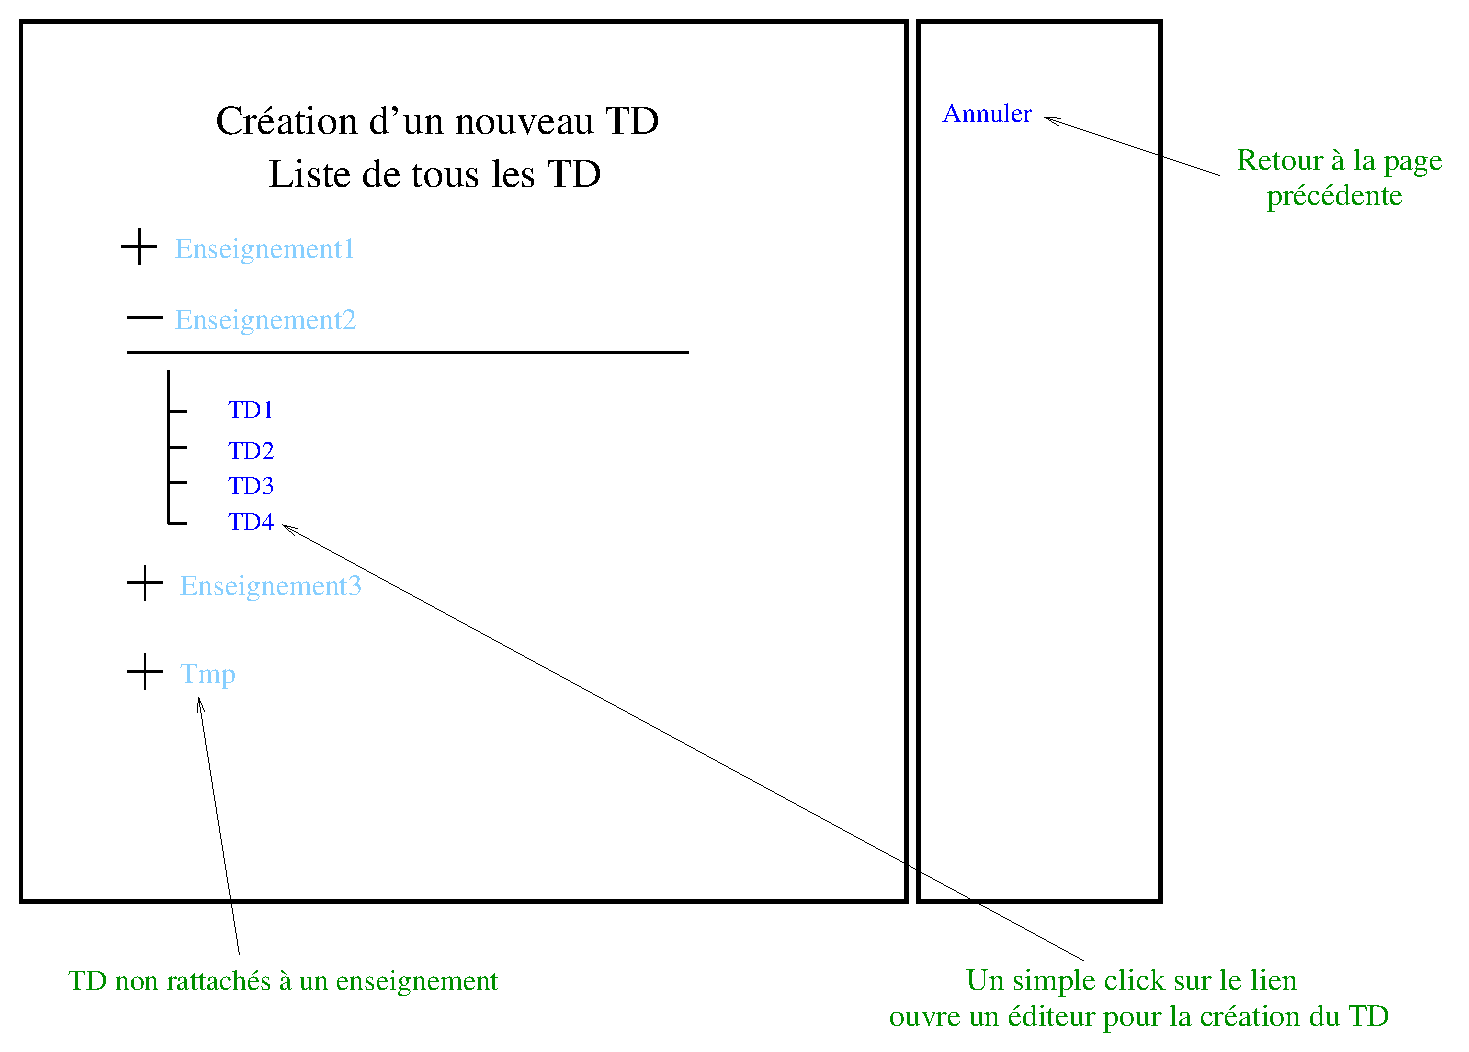
\includegraphics{../eps/CreerTDAncien_Listing.eps}}\\
{\it Listing des TD existants dans la base, tri�s par enseignements}
\end{flushleft}
\newpage
\subsection{Nouveau TD}
Il existe deux mani�res de cr�er un nouveau TD:
\begin{itemize}
\item Soit l'enseignant importe un fichier XML depuis son compte.
\item Soit il �dite directement le TD dans l'�diteur de bord.
\end{itemize}

\begin{flushleft}
\scalebox{0.5}{\includegraphics{../eps/CreerNewTDMain2.eps}}\\
{\it Page principale lors de la cr�ation d'un nouveau TD}
\end{flushleft}

\subsection{Editeurs de bord}
Plusieurs vues sont propos�es � l'enseignant pour �diter son TD.
\begin{itemize}
\item La vue Delta
\item Le fichier XML avec les balises.
\item Une version texte sans balise XML.
\end{itemize}

L'enseignant utilise pour la saisie du TD l'�diteur embarqu�, dans la zone de visualisation.

Il existe trois mani�res d'�crire le TD.


\begin{flushleft}
\scalebox{0.5}{\includegraphics{../eps/tdEditionBalise.eps}}\\
{\it L'enseignant saisie le TD soit directement en XML soit en mode texte}
\end{flushleft}

\begin{flushleft}
\scalebox{0.5}{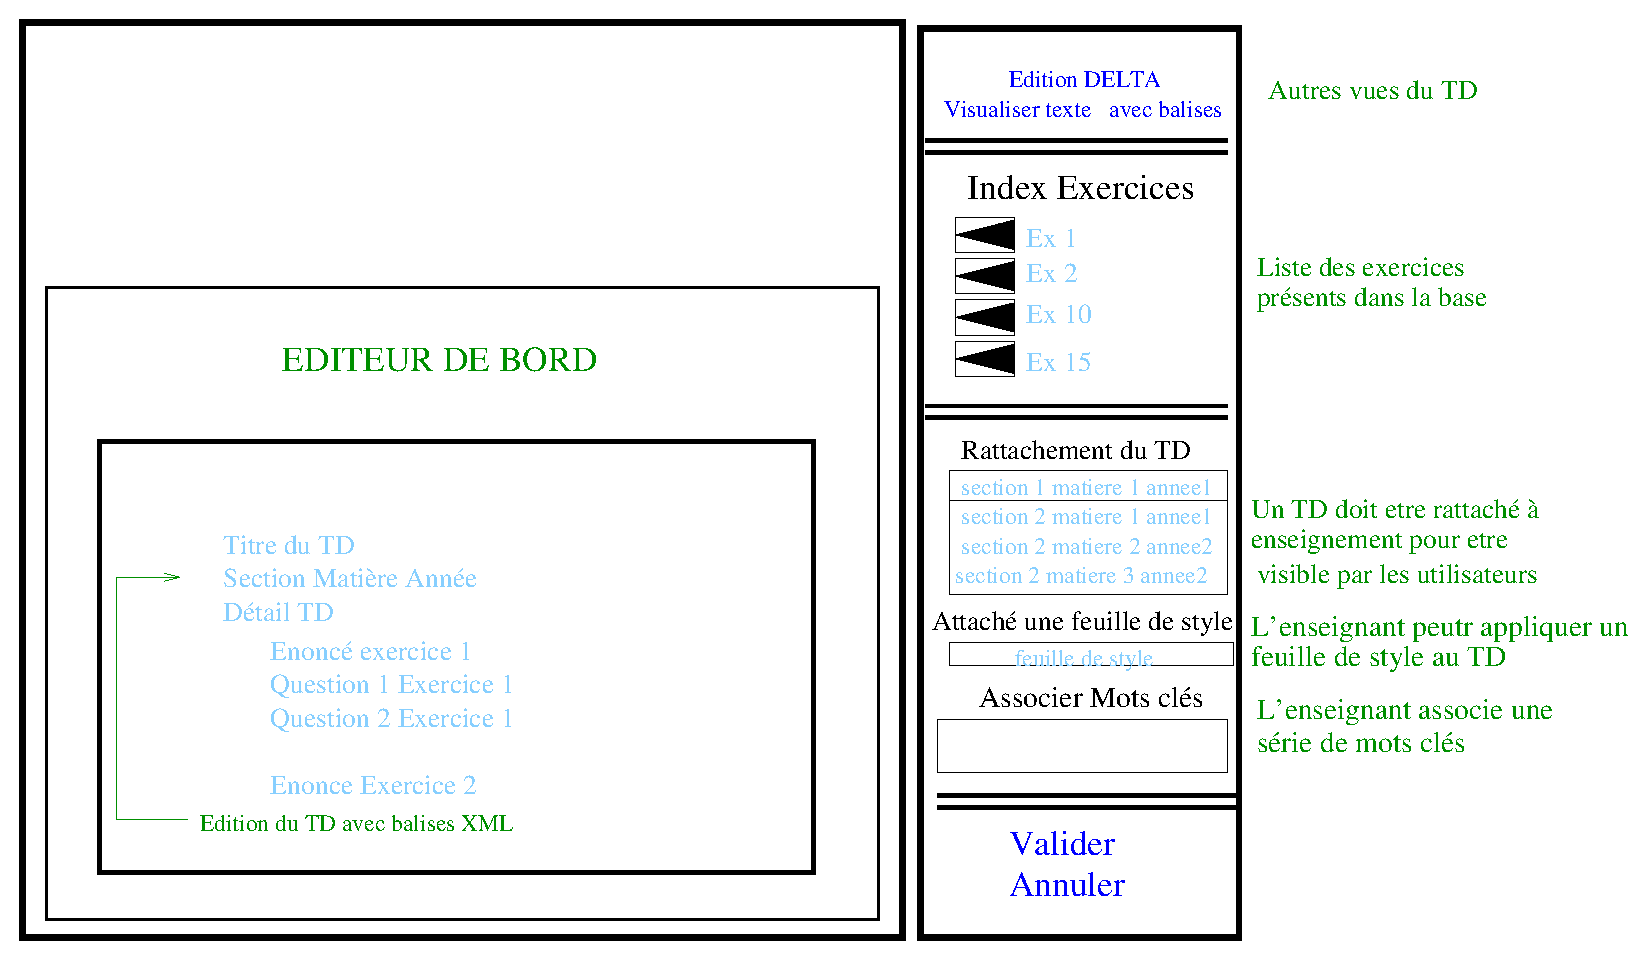
\includegraphics{../eps/tdEditionSansBalise.eps}}\\
\end{flushleft}
\newpage
La derni�re propose� est la  vue Delta. Cette vue consiste � lister le contenu du TD courant dans la zone de visualisation.
Dans la zone annexe, l'enseignant a acc�s � la liste des exercices qui existent dans la base.
Depuis l'index des exercices, l'enseignant s�lectionne un exercice et l'ajoute au TD avec la fl�che gauche.
Il peut modifier l'ordre des exercices � l'int�rieur du TD avec les deux fl�ches (Haut Bas)
Il peut �galement retirer un exercice du TD qu'il construit avec la fl�che droite.
Une fois le TD construit, pour diffus� le TD il doit le rattacher � un enseignement.
S'il ne le rattache pas, le TD ne sera pas visible pour les
consultants et sera stock� dans un r�pertoire temporaire.
\begin{flushleft}
\scalebox{0.5}{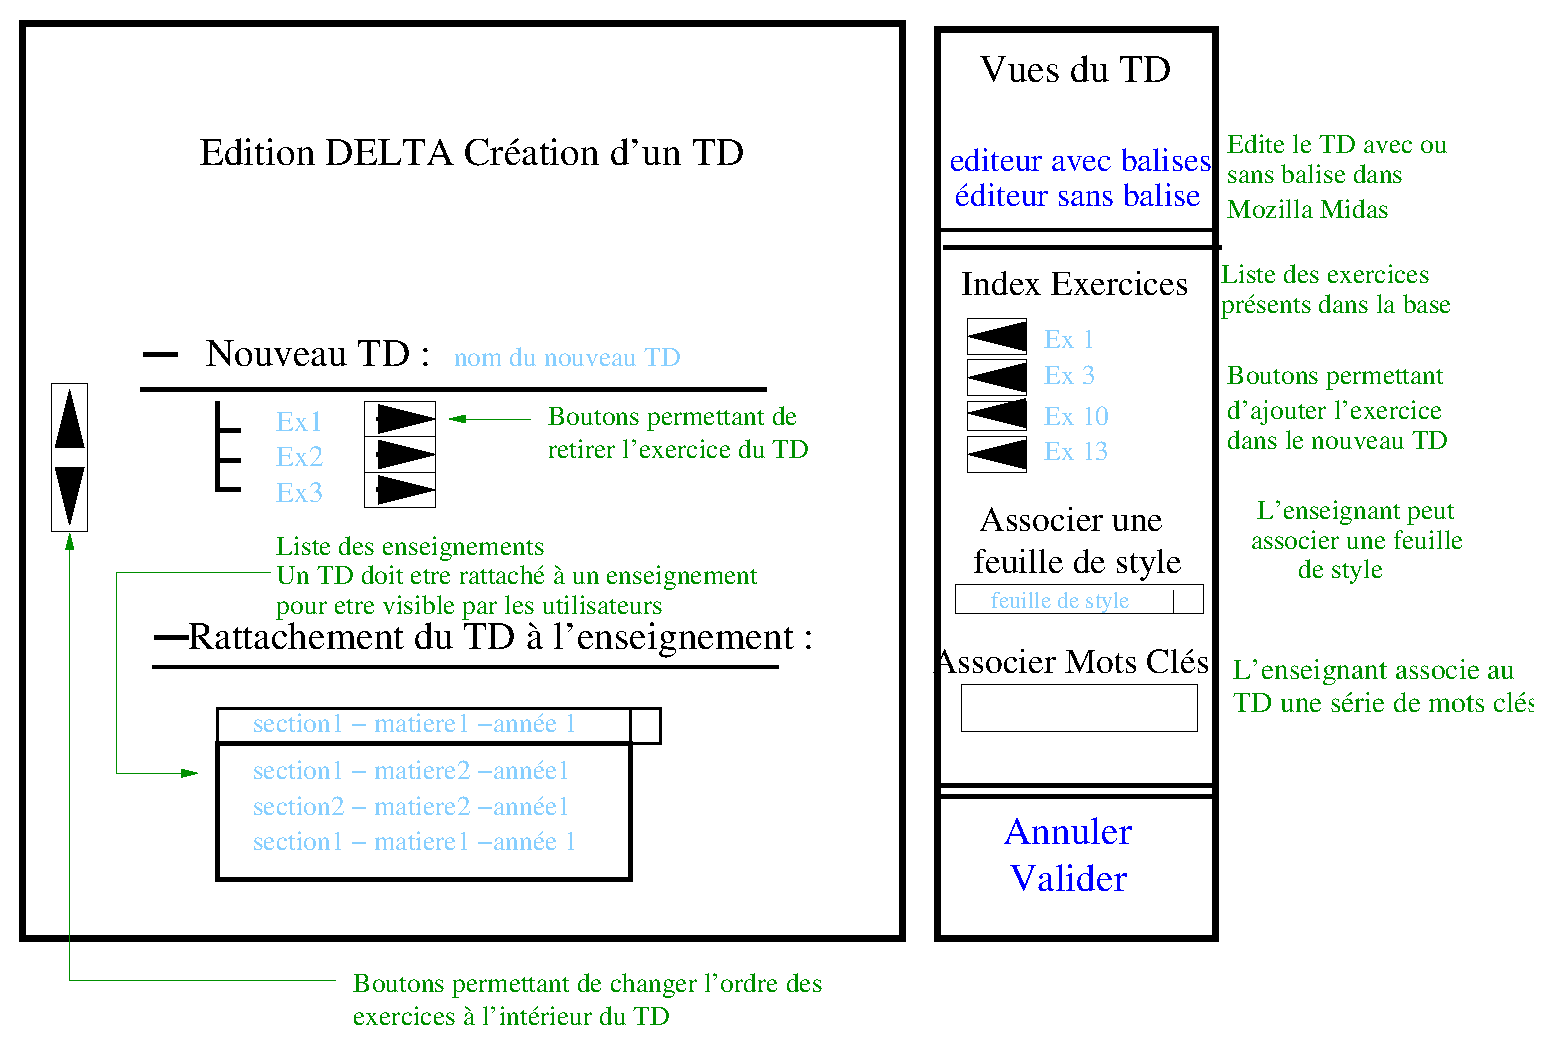
\includegraphics{../eps/tdCreerPanier.eps}}\\
{\it Vue Delta}
\end{flushleft}

L'enseignant enregistre son TD.